%%%%%%%%%%%%%%%%%%%%%%%%%%%%%%%%%%%%%%%%%%%%%%%%%%%%%%%%%%%%%%%%%%%%%%%%%%%%%%%
% Chapter 4: Título del capítulo 4
%%%%%%%%%%%%%%%%%%%%%%%%%%%%%%%%%%%%%%%%%%%%%%%%%%%%%%%%%%%%%%%%%%%%%%%%%%%%%%%

\section{Introducción}
\label{4:sec1}

Con vistas a probar y testear que todo funcionaba de forma correcta, Casiano me sugirió probar la plataforma para la realización de algunas prácticas individuales y grupales.
Por ello, decidimos realizar algunas tareas para la asginatura de Procesadores de Lenguajes en CodeLab.

\section{Detección de errores}
\label{4:sec2}

Al poner en uso la plataforma, los alumnos de Procesadores de Lenguajes nos ayudaron a encontrar algunos errores:

\begin{itemize}
    \item Imposibilidad de crear repositorios privados
    \item No se añadía el usuario como colaborador al repositorio.
\end{itemize}

Los alumnos utilizaron la funcionalidad de los issues para notificar el error añadiendolos en el repositorio.

Todas los errores fueron solucionados lo más rápido posible para que los alumnos de Procesadores de Lenguajes pudiesen usar la plataforma de forma correcta y realizar sus tareas en su repositorio correspondiente.
Por tanto, CodeLab se comenzó a usar en producción en un aula de 31 alumnos, demostrando que es una herramienta totalmente funcional y capaz de gestionar las tareas de código de una asignatura.

\begin{figure}[!th]
\begin{center}
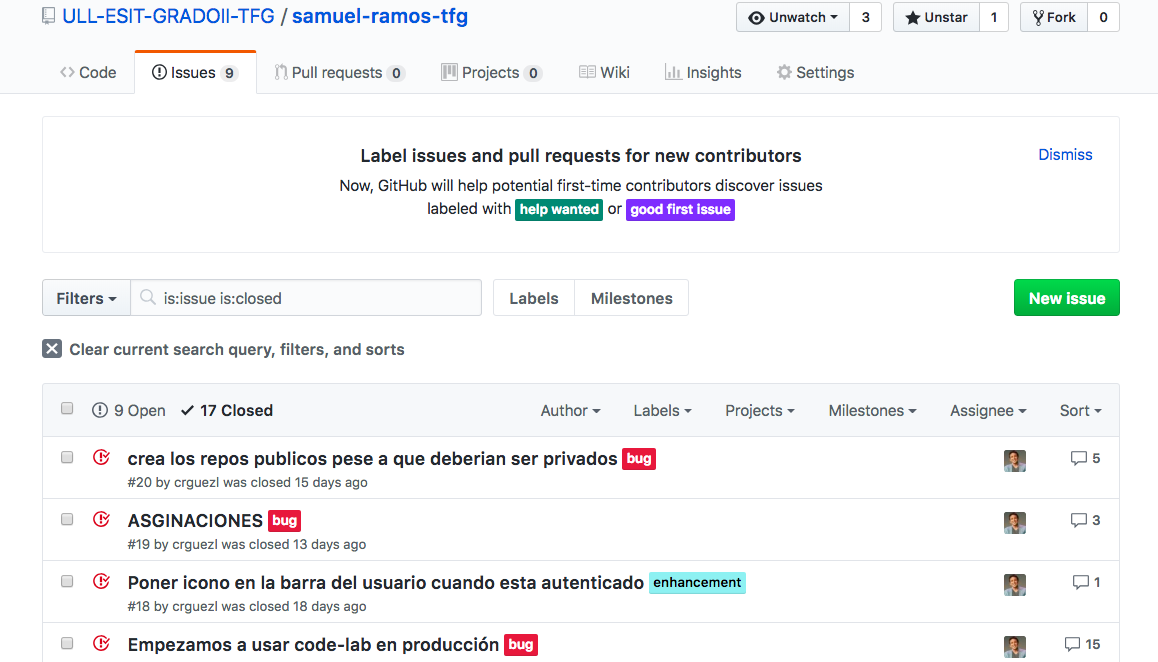
\includegraphics[scale=0.5]{images/issues}
\caption{Incidencias Cerradas }
\label{fig:issues}
\end{center}
\end{figure}

\newpage

Aparte de errores, Casiano encontró varias mejoras que podrían ser útiles para la plataforma:

\begin{itemize}
    \item Foto y nombre del usuario en la barra de navegación.
    \item Ubicación del profesor, es decir, especificar si se encuentra en un aula o en una tarea.
    \item Elección de permisos del alumno dentro del repositorio de Github.
    \item Algunos fallos visuales como sombreados que impedían que el texto se viese de forma correcta.
\end{itemize}


Las mejoras fueron valoradas y realizadas para mejorar la interfaz gráfica y pulir ciertos defectos básicos.
Sin el test de un profesor estos defectos y mejoras hubiesen sido más complicados de encontrar y resolver.
